\chapter{Background}

This chapter provides a review of the current research on Deep Neural Networks, their optimization techniques and the state of art results for image recognition. Optimization methods will be first discussed followed by current DNN architectures.

\section{ (Shallow) Neural Networks}

In the context of machine learning, Neural Networks are a class of differentiable algorithms \cite{bishop1995neural}. One can think of them as a set of perceptrons aligned into several layers having outputs from layer \textit{L} mapped to inputs of the layers \textit{L+1}. The output of each perceptron is named activation and the set of activations in the final layer gives the desired classification output. For each connection, a neuron has one weight connecting with all neurons of the next/previous layer, and one bias. The goal is to find the values that minimizes a given cost function. For instance a network could have 10 neurons in the last layer that would map to a digit classification problem using the MNIST \cite{lecun1998mnist} dataset. The neurons from 1-10 on this layer corresponds to each number, and the one with the highest activation value would be chosen as the classification output.

\begin{figure}[h!]
\centering
	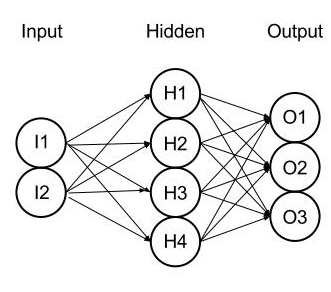
\includegraphics[scale=0.5]{mlnet.png}
\caption{Multi-layer Perceptron}
\label{fig:mlnet}
\end{figure}


\section{Gradient Methods and Backpropagation}

As most machine learning algorithms, Neural Networks models rely on optimizations of weights $\omega$ and biases $\beta$. In order to calculate these values one should  choose a cost function that measures the variance between the actual result and the desired output on each iteration of the training phase. The two methods for running this optimization algorithm on Neural Networks are known as \textit{Backpropagation} and \textit{Gradient Descent} \cite{goodfellow2016_book}. The main goal of the algorithm is to propagate small changes $\delta$ applied to any of the neurons of the network all the way to the final layer.

\begin{figure}[h!]
\centering
	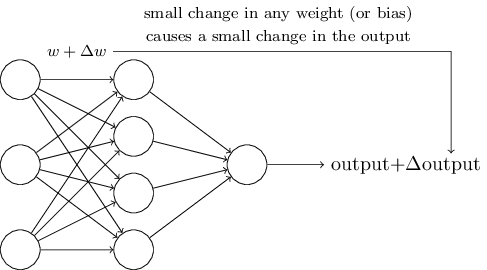
\includegraphics[scale=0.5]{net_change.png}
\caption{Output change with regards to layer(s) weight change \cite{nielsen2016}}
\label{fig:net_change}
\end{figure}


The network learns from data using convex optimization techniques that involves calculating derivatives of linear and polynomial cost functions.The learning algorithm should be able to find weights and biases that best approximates the output \textit{y(x)}. This approximation consists of finding the global minimum of a chosen cost function. Different machine learning algorithms require different cost functions \cite{nielsen2016}. Ultimately, one should be interested in calculating the change on the cost with respect to the weights and biases of all the neurons. This calculation makes use of partial derivatives with respect to the $\omega$ and $\beta$ in order to find the direction of the minimum for a given function $f(x)$, namely gradient \cite{goodfellow2016_book}.

$$\nabla C \equiv \frac{\partial C}{\partial \omega}, \frac{\partial C}{\partial b}$$

Gradient Descent is one of the methods for finding a global/local minimum of a function. This calculation yields what is a called a gradient vector $\nabla$C which is subtracted from current weight and biases on each iteration in order to move the result towards the global or local minimum. The gradient calculation can be seen as repeatedly computing $\nabla$C, and then moving in the opposite direction "falling down" the slope of the valley.

\begin{figure}[!ht]
\centering
	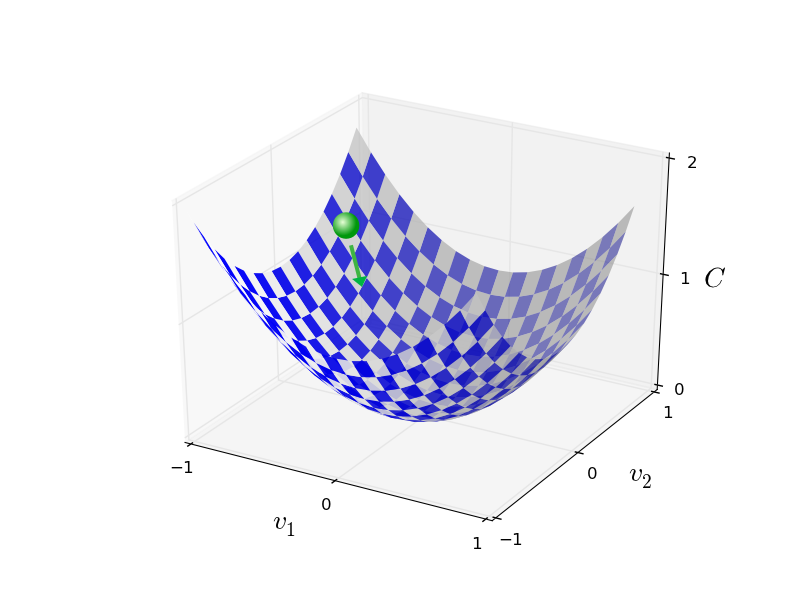
\includegraphics[scale=0.3]{valley_with_ball.png}
\caption{Gradient calculation representation \cite{nielsen2016}}
\label{fig:net_change}
\end{figure}
In order to learn the best representation of a given data set a Neural Network should go through the optimization process where each data point is used many times to estimate the network current weights and biases. Each iteration pushes the ball into the direction of the valley by comparing a given y($x_n$) with its corresponding real $y_n$. The process should be stopped when the ball hits the lowest point of the valley, in other words, when the algorithm has converged. Mathematically speaking this is known as reaching a minimum of a function \cite{nielsen2016}. Some optimization problems are unable to find a global minimum due to their complexity, on this case, convergence is achieved by finding the local minimum.

However, when the data set is too big for running one update after a complete loop over the entire data, one should come with better strategy for updating the network parameters. Such method is that where each iteration runs on a subset of the training input namely \textit{Stochastic Gradient Descent}. One of the biggest advantages is that to speed up learning while the estimation of the gradient $\nabla$C is being computed over a subset of the data instead of all training inputs. The subset is chosen randomly on every iteration and can be referred as mini-batch. These batches are selected every \textit{epoch} and the user provides how many epochs the algorithm should run. Due to the large amount of parameters, neural networks used in Deep Learning make use of this method so training can happen within feasible time frames.


The training is comprised mainly of two different types of calculations: Feedforward and Backpropagation. Feedforward is the starting point of the network weights and biases optimization.The goal is to calculate the activation of each neuron from the first layer to the output layer. It involves evaluating the activation function with respect to the current weights and biases of the network by forward-propagating \textit{x} through the entire architecture. This operations yields an error $\delta$, which triggers the backpropagation part. When feedforward reaches the last layer, the error is then calculated and backpropagated to the L-1 layer. For each layer, one should find the rate of change of the cost function for each of the weights and biases with respect to its neurons. This operation is repeated subsequently until the first input layer, where the current "belief" of the network is updated making it ready for another feedforward calculation. The overall process should stop when there is no relevant changes in the output of the cost function.

\section{Convolutional Neural Networks}

Convolutional Networks are a class of deep learning algorithms that can use many layers of nonlinear or linear processing in cascade for feature extraction and transformation. They are still very similar to ordinary Neural Networks (made up of neurons that have learnable weights and biases). However, such algorithms makes the explicit assumption that the inputs are images and, therefore, are based on learning abstract representations of data with spatial properties \cite{goodfellow2016_book}. For example, an image could be represented by a vector of intensity values from 0-255 for each pixel and after being processed by the first layers of a Convolutional Neural Network those would become more abstract representation such as set of edges, regions of particular shape and etc \cite{stanford2016}.

A convolutional neural network is different from the traditional neural network. Instead of connecting each pixel of an image, for instance, to all the neurons in the next layer, groups of pixels of fixed sizes known as patches, are connected to different groups of neurons. Each group specializes in learning specific features from the data and are not necessarily connected with all other groups in the current or next layer. The input region or group of neurons connected to a patch in the image is known as local receptive field \cite{nielsen2016}. The main advantage over shallow architectures is that the latter does not take into account the inherent spatial structure of images, in other words, all pixels are treated equally.

The main architectural difference of ConvNets is that they have added some different layers to the traditional Neural Nets mix. The name "convolutional" originates from the Convolution layer which is responsible for computing the output of neurons that are connected to local regions in the input. This operation is commonly referred in image/signal processing as a convolution between two matrices/vectors of variable sizes. The smaller regions in which the image is connected is referred as filters and/or kernels, and these would be responsible for detecting abstract features on different regions of a picture for instance. After each sequence of convolutional layers there are also the Pooling Layers. The main goal is to perform downsampling operation along spatial dimensions of an image (i.e width and height). This is important as an image with higher dimensions will be reduced at each layer forcing the network to learn deeper and deeper features at each iteration.

\begin{figure}[!h]
\centering
	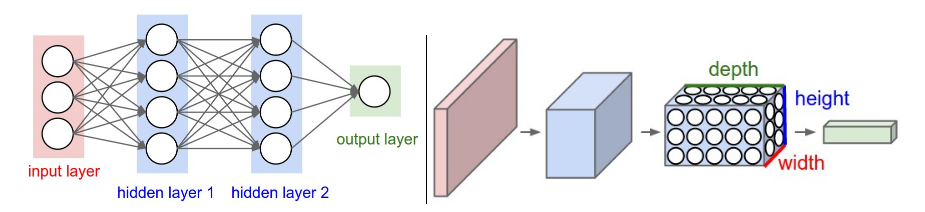
\includegraphics[scale=0.6]{conv.png}
\caption{Shallow Neural Network vs Convolutional Neural Network}
\cite{stanford2016}
\label{fig:conv}
\end{figure}

Convolutional Neural Networks are considered the state of the art solution for computer vision problems. The archutecture developed by Krizhevsk et al. (2012) achieved an averaged top-1 and top-5 test set error rates of 37.5\% and 17\% where the previously record was 45.7\% and 25.7\% by a different technique. The network was comprised of eight layers, 5 of which were convolutional layers and the remaining were three fully connected layers. The output of the three last layers was fed to a 1000-way softmax to produce 1000 different image classes labels of the ImageNet dataset. Besides, max-pooling layers were also used following the fifth convolutional layer and response-normalization layers. Adding or removing any layers on this architecture yielded worst results. Overfitting was treated by using both Data Augmentation and Dropout \cite{hinton2012improving} techniques since the architecture had over 60 million parameters. These results show that deep convolutional networks are capable of achieving above the average results even when challenging datasets with several classes are used.
\section{CNN Feature Learning and Visualization}

Visualizing the features of a convolutional layer helps one to understand what are the main characteristics of the input that are not only being learned but are also responsible for maximizing neurons activations cite{zeiler2014visualizing}. Until recently there was no clear understanding of why Convolutional Networks perform so well on image classification tasks. Zeiler et al (2014) have produced a novel visualization technique that gives insights into the outputs of the intermediate feature layers of the network. These visualizations were then used to perform diagnostics of models and, thus, find architectures that can outperform current state of the art algorithms. One can understand that all the convolutional layers are in fact "feature extraction" layers while the fully connected ones are the actual classifier.

\begin{figure}[!h]
	\centering
	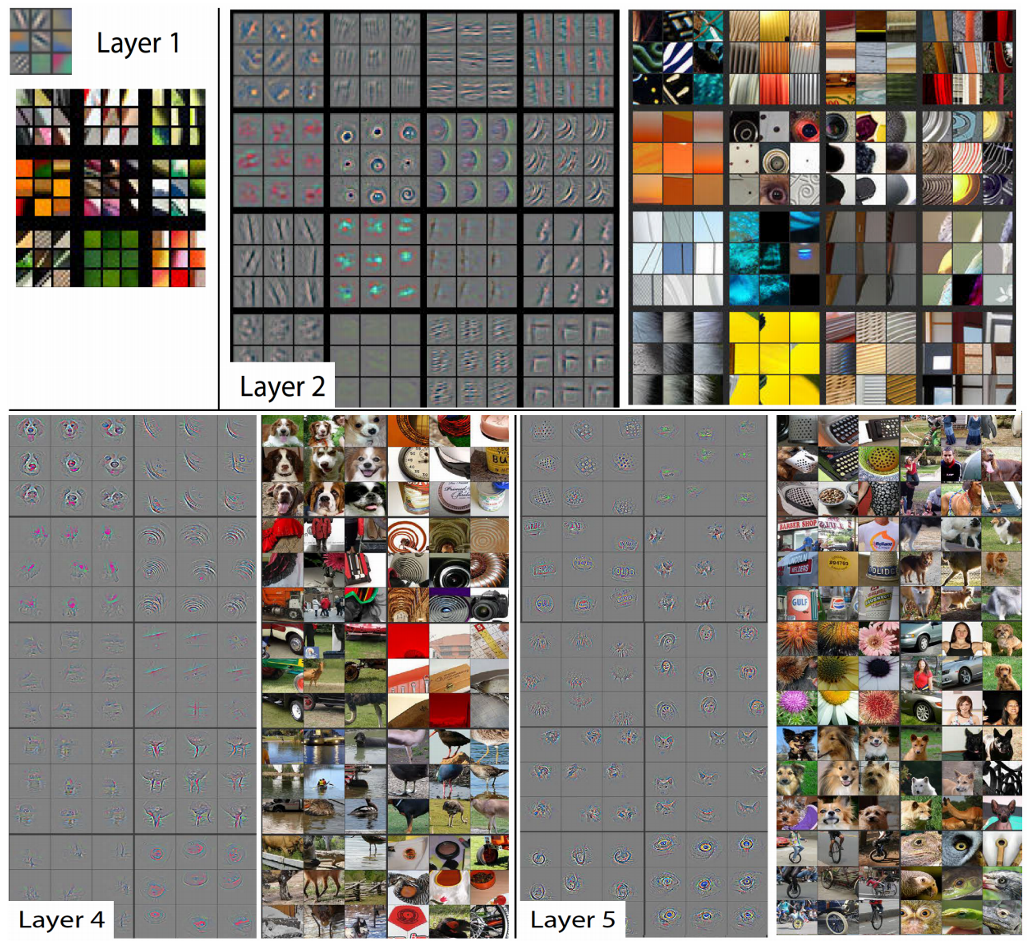
\includegraphics[scale=0.6]{layer_vis.png}
	\caption{CNN layer visualization}
	\cite{zeiler2014visualizing}
	\label{fig:conv_layer_vis}
\end{figure}

Features are learned from more abstract on initial layers to more specific and concrete on deeper layers. Figure ~\ref{fig:conv_layer_vis} shows that the first neurons are learning different types of edges while later neurons are capable of learning full representations of important regions of an image. In general these features are applicable to many datasets and tasks. As features transition from general to specific, transferability becomes negatively affected \cite{yosinski2014transferable}. For instance two similar datasets as the ImageNet and Cifar10 would share many common features and, therefore, a network trained on one, could be used as a pre training or weight initialization process for another, increasing the generalization and accuracy of the model.
\section{CNN Architectures}

The use of Deep Neural Networks (DNNs) as a prominent technique was mainly possible due to the standardization of the dataset used for such tasks. ImageNet has become the most used classification challenge for those wanting to find better CNN architectures. The main goal of such challenges are to find models with better accuracies without focusing too much on resource utilisation. One one hand, the most important metric of a good machine learning model is its accuracy, in other words, how well it can generalize on different datasets. On the other hand, several other important metrics should be taken into consideration when using an specific DNN system in real life such as: memory footprint, parameters, operations count and etc \cite{canziani2016analysis}.

\begin{figure}[!h]
	\centering
	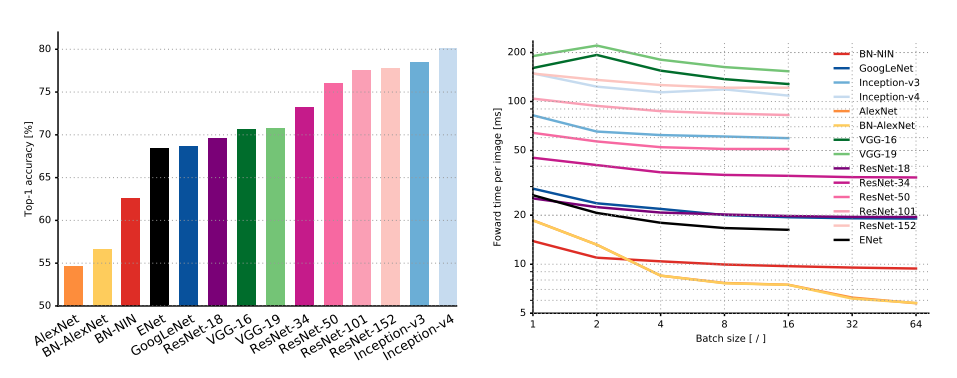
\includegraphics[scale=0.6]{network_comparison.png}
	\caption{(Left) Accuracy of Different CNN models (Right) Inference time for different batch sizes}
	\cite{canziani2016analysis}
	\label{fig:cnn_comparison}
\end{figure}

As new methods develop, one should always pick the one that is capable of not only learning the features of the target domain but also would fit the resource capacity of the system. From one of the first CNN architectures (AlexNet) to the latest models (Inception V4), the accuracy has improved from $55\%$ to almost $80\%$ on the ImageNet dataset (comprised of 1.000 different class labels).

\section{Deep Neural Networks Properties}\label{subsec: nn_props}

Deep Neural networks can be considered models with high expressiveness that can achieve extremely good performance on computer vision tasks. At the same time that being highly expressive helps them to succeed, it also drives them to learn solutions that are not easily understandable \cite{szegedy2013}. Usually there is a discontinuity in the input-output mappings of neural networks which can lead to miss-classification of images when the network prediction error is maximized \cite{gu2014}.The learning process of these networks through the use of backpropagation is rather complex and sometimes difficult to understand.

In order to visualize the semantic meaning of individual units, studies are currently focusing on understanding the factors leading to the activation of network neurons. It has been argued that deep neural networks should be stable enough to provide robustness to small perturbation of its inputs \cite{szegedy2013}. However, it has been found by mainly Goodfellow et al. (2014) and Szegedy et al. (2013) that minimal local perturbations can indeed affect the network's predictions bringing down the assumption that DNN have very good local generalization. Methods for exploiting this vulnerability were created and proven to be effective by having a very high confidence classification of adversarial examples \cite{goodfellow2016}.

Generalization is usually achieved by making non-local assumptions of the training inputs. Deep stacks of non-linear layers are one of the ways to have the model encoding a non-local generalization prior over the input space \cite{gu2014}. Therefore, output units should be able to assign low probabilities to regions of the input space where no training examples are found within its vicinity. The representation of low-probability "pockets" of space on images can lead to the creation of Adversarial examples. These are created by adding small localized perturbations on the input space which can ultimately lead to the wrong classifier outcome. 


The following sections are going to focus on Adversarial Examples and how the exploitation of the aforementioned network properties can be used to craft such examples. Three methods will be presented along with results found by different studies. Finally, methods for using this adversarial information for regularizing networks will also be shown as a possible solution for making deep neural networks less vulnerable to these kind of attacks.

\section{Learning from imbalanced data}
In general, machine learning algorithms are designed to assume that the number of samples in a specific class label are roughly similar. Nevertheless, this scenario is often rare on the real world, as in most cases, the data distribution available is skewed and, hence, causes the model to be biased towards the labels with higher number of data points. This problem domain is often known as learning from imbalanced data \cite{japkowicz2002class} and points to critical questions that are yet to be answered so one can gain deeper understanding of the vast field of machine learning. Generally speaking, there are three main approaches to learning from imbalanced data \cite{krawczyk2016learning}. 
\begin{itemize}
	\item Data-level: Aims to manipulate the data distribution by performing oversampling and undersampling operations to make it suitable for a standard learning algorithm
	\item Algorithm-level: Concentrates on modifying existing techniques to prevent bias towards majority classes and incorporate, for instance, varying penalties for each individual group of examples.
	\item Hybrid: Combines the advantages of the two previous approaches.
\end{itemize}

Even though there has been continuous development on learning from imbalanced data, there are still some new emerging challenges in, more specifically, highly dimensional data domains. As the number of dimensions of the training dataset grows, the difficulty into occupying the data space properly also increases. Varied forms of learning such as supervised, unsupervised and regression suffer from data imbalance. Moreover, extensive research on real-life applications shows that uneven data representation is an ongoing problem \cite{krawczyk2016learning}.
